\subsection{Deep Gated Network : Decoupling Gates and Weights}\label{sec:dgn}
Note that since $\hat{y}_{\Theta}(x)=\ip{\phi_{x,\Theta},v_{\Theta}}$, during training, as $\Theta$ is learnt, both the NPFs and NPV are also learnt. Hence, in order to understand the roles of $\phi_{x,\Theta}$ and $v_{\Theta}$ it is a good idea to separate them. This is achieved by the deep gated network (DGN) setup (see \Cref{fig:dgn}), which has two networks namely the \emph{feature network} parameterised by $\Tf\in\R^{d^{\text{f}}_{\text{net}}}$ which holds the NPFs (i.e., the gating information) and a \emph{value network} parameterised by $\Tv\in\R^{d^{\text{v}}_{\text{net}}}$ which holds the NPV.  The combined parameterisation is denoted by $\Theta^{\text{DGN}}=(\Tf,\Tv)\in \R^{d^{\text{f}}_{\text{net}}+d^{\text{v}}_{\text{net}}}$.  
\FloatBarrier
\begin{figure}[h]
\centering
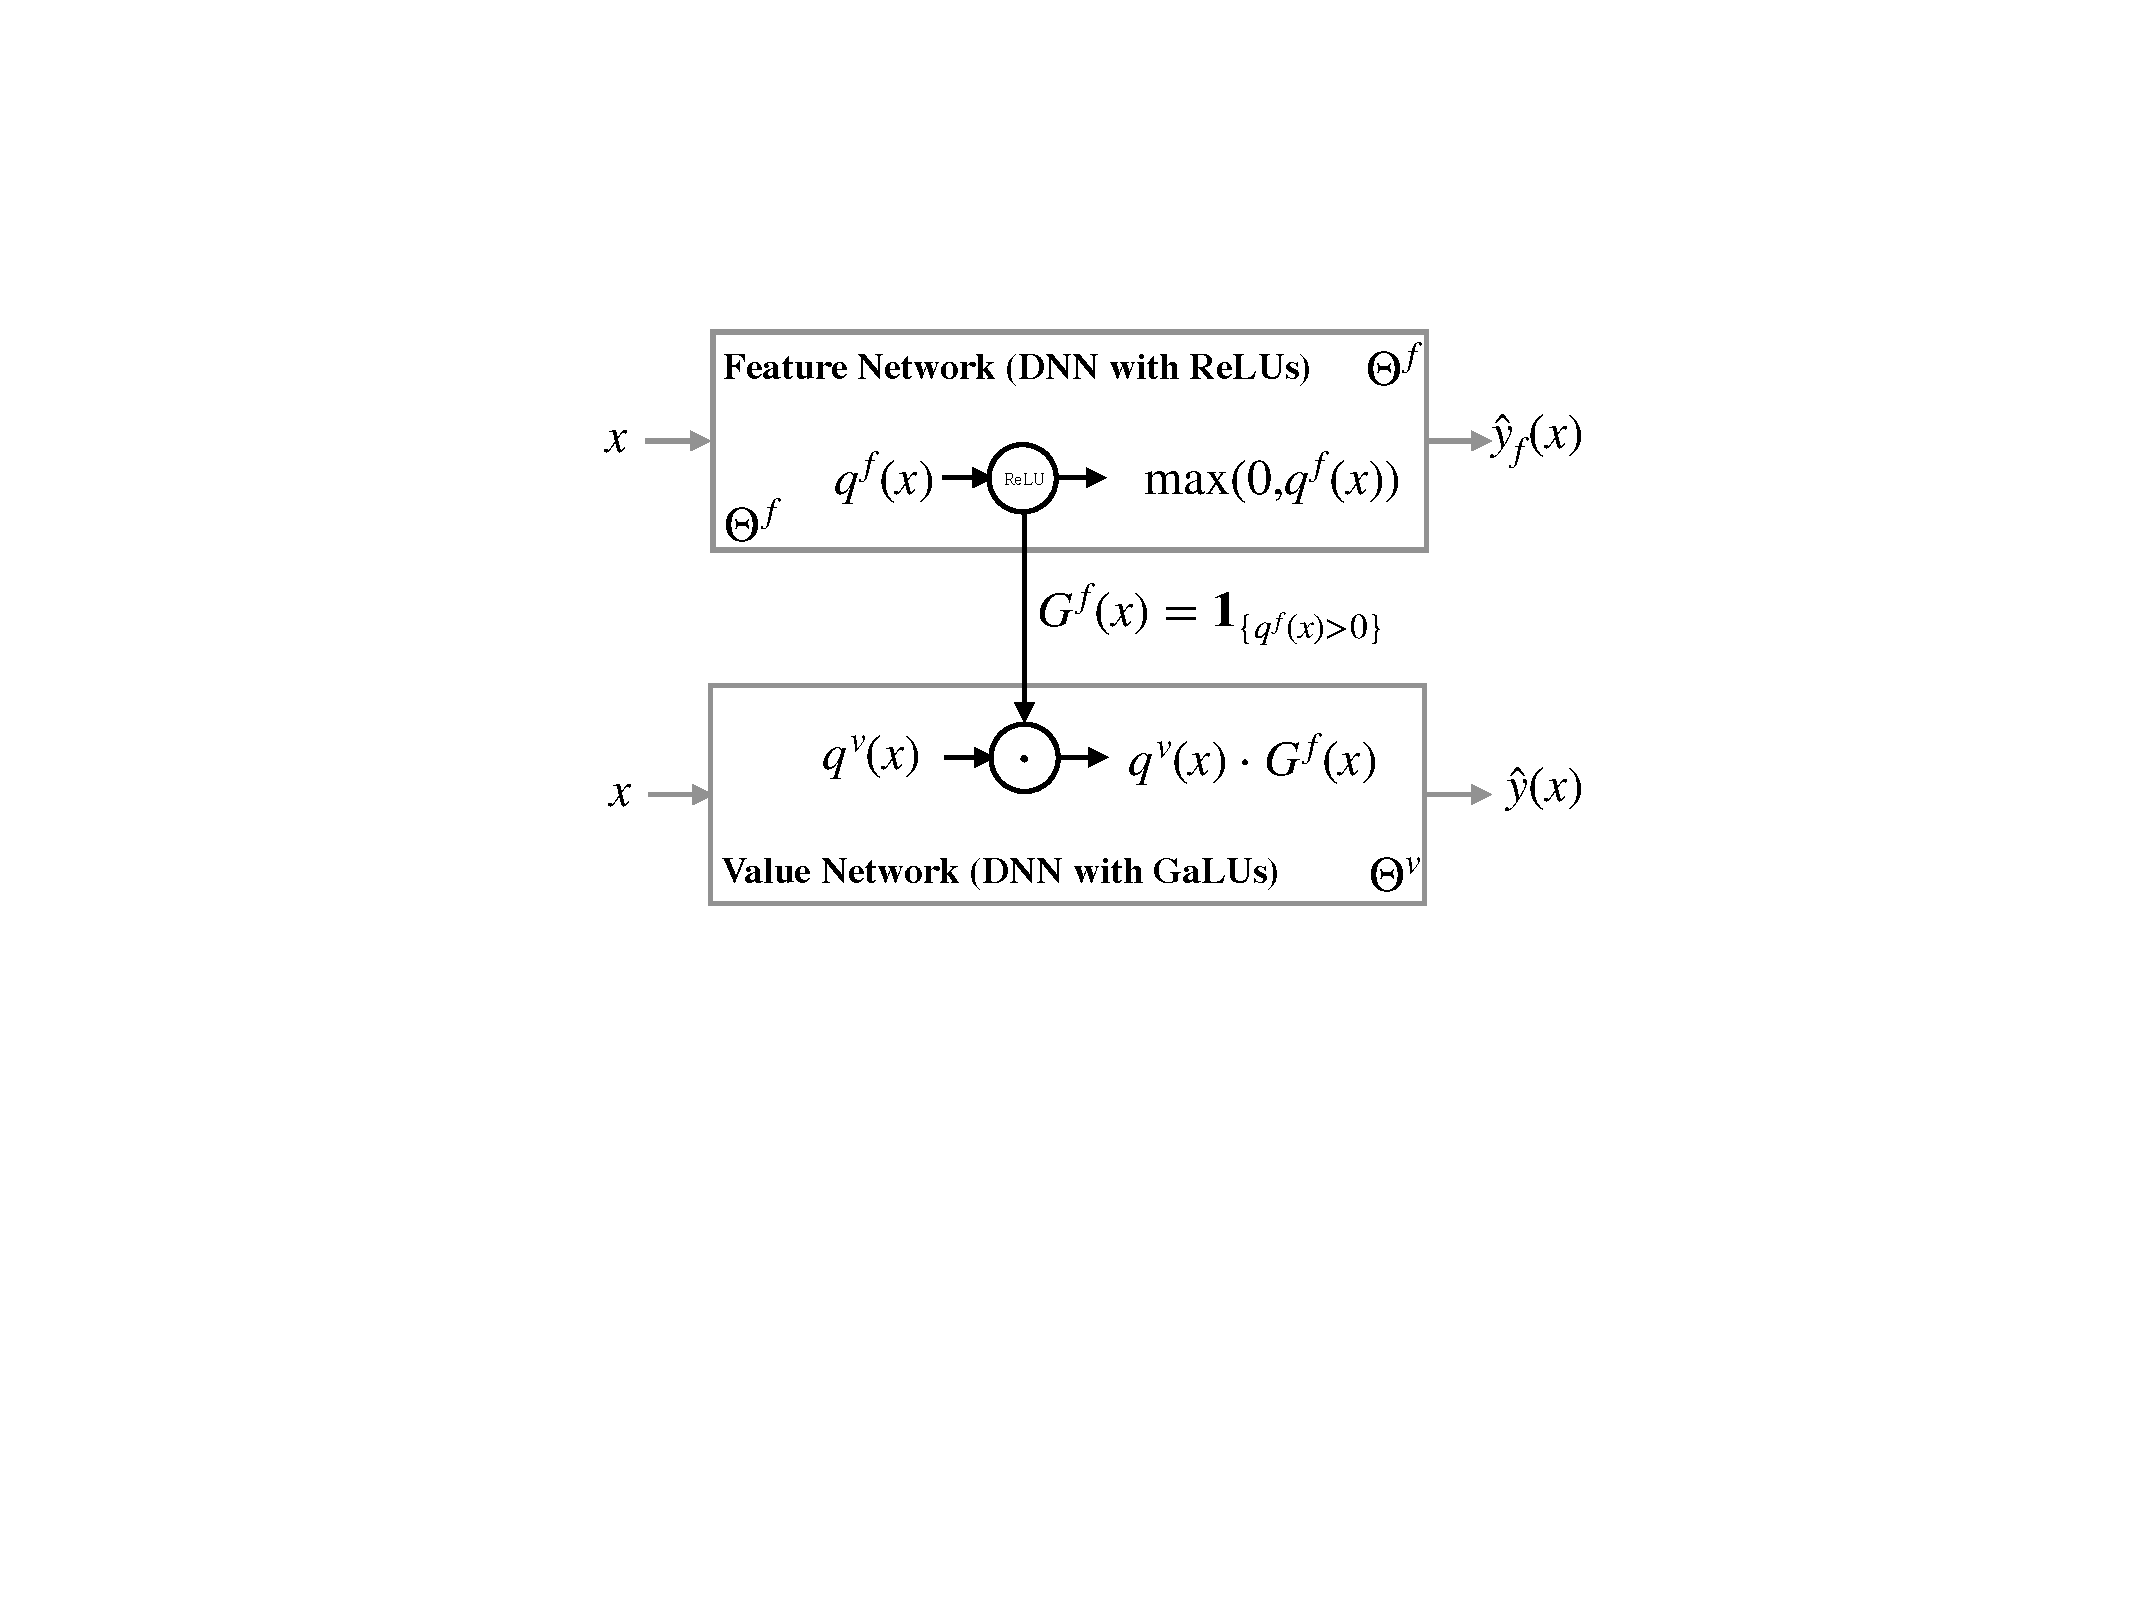
\includegraphics[scale=0.25]{figs/dgn-nips.pdf}
\caption{Deep Gated Network }
\label{fig:dgn}
\end{figure}
\begin{comment}
\FloatBarrier
\begin{figure}[h]
\begin{minipage}{0.35\columnwidth}
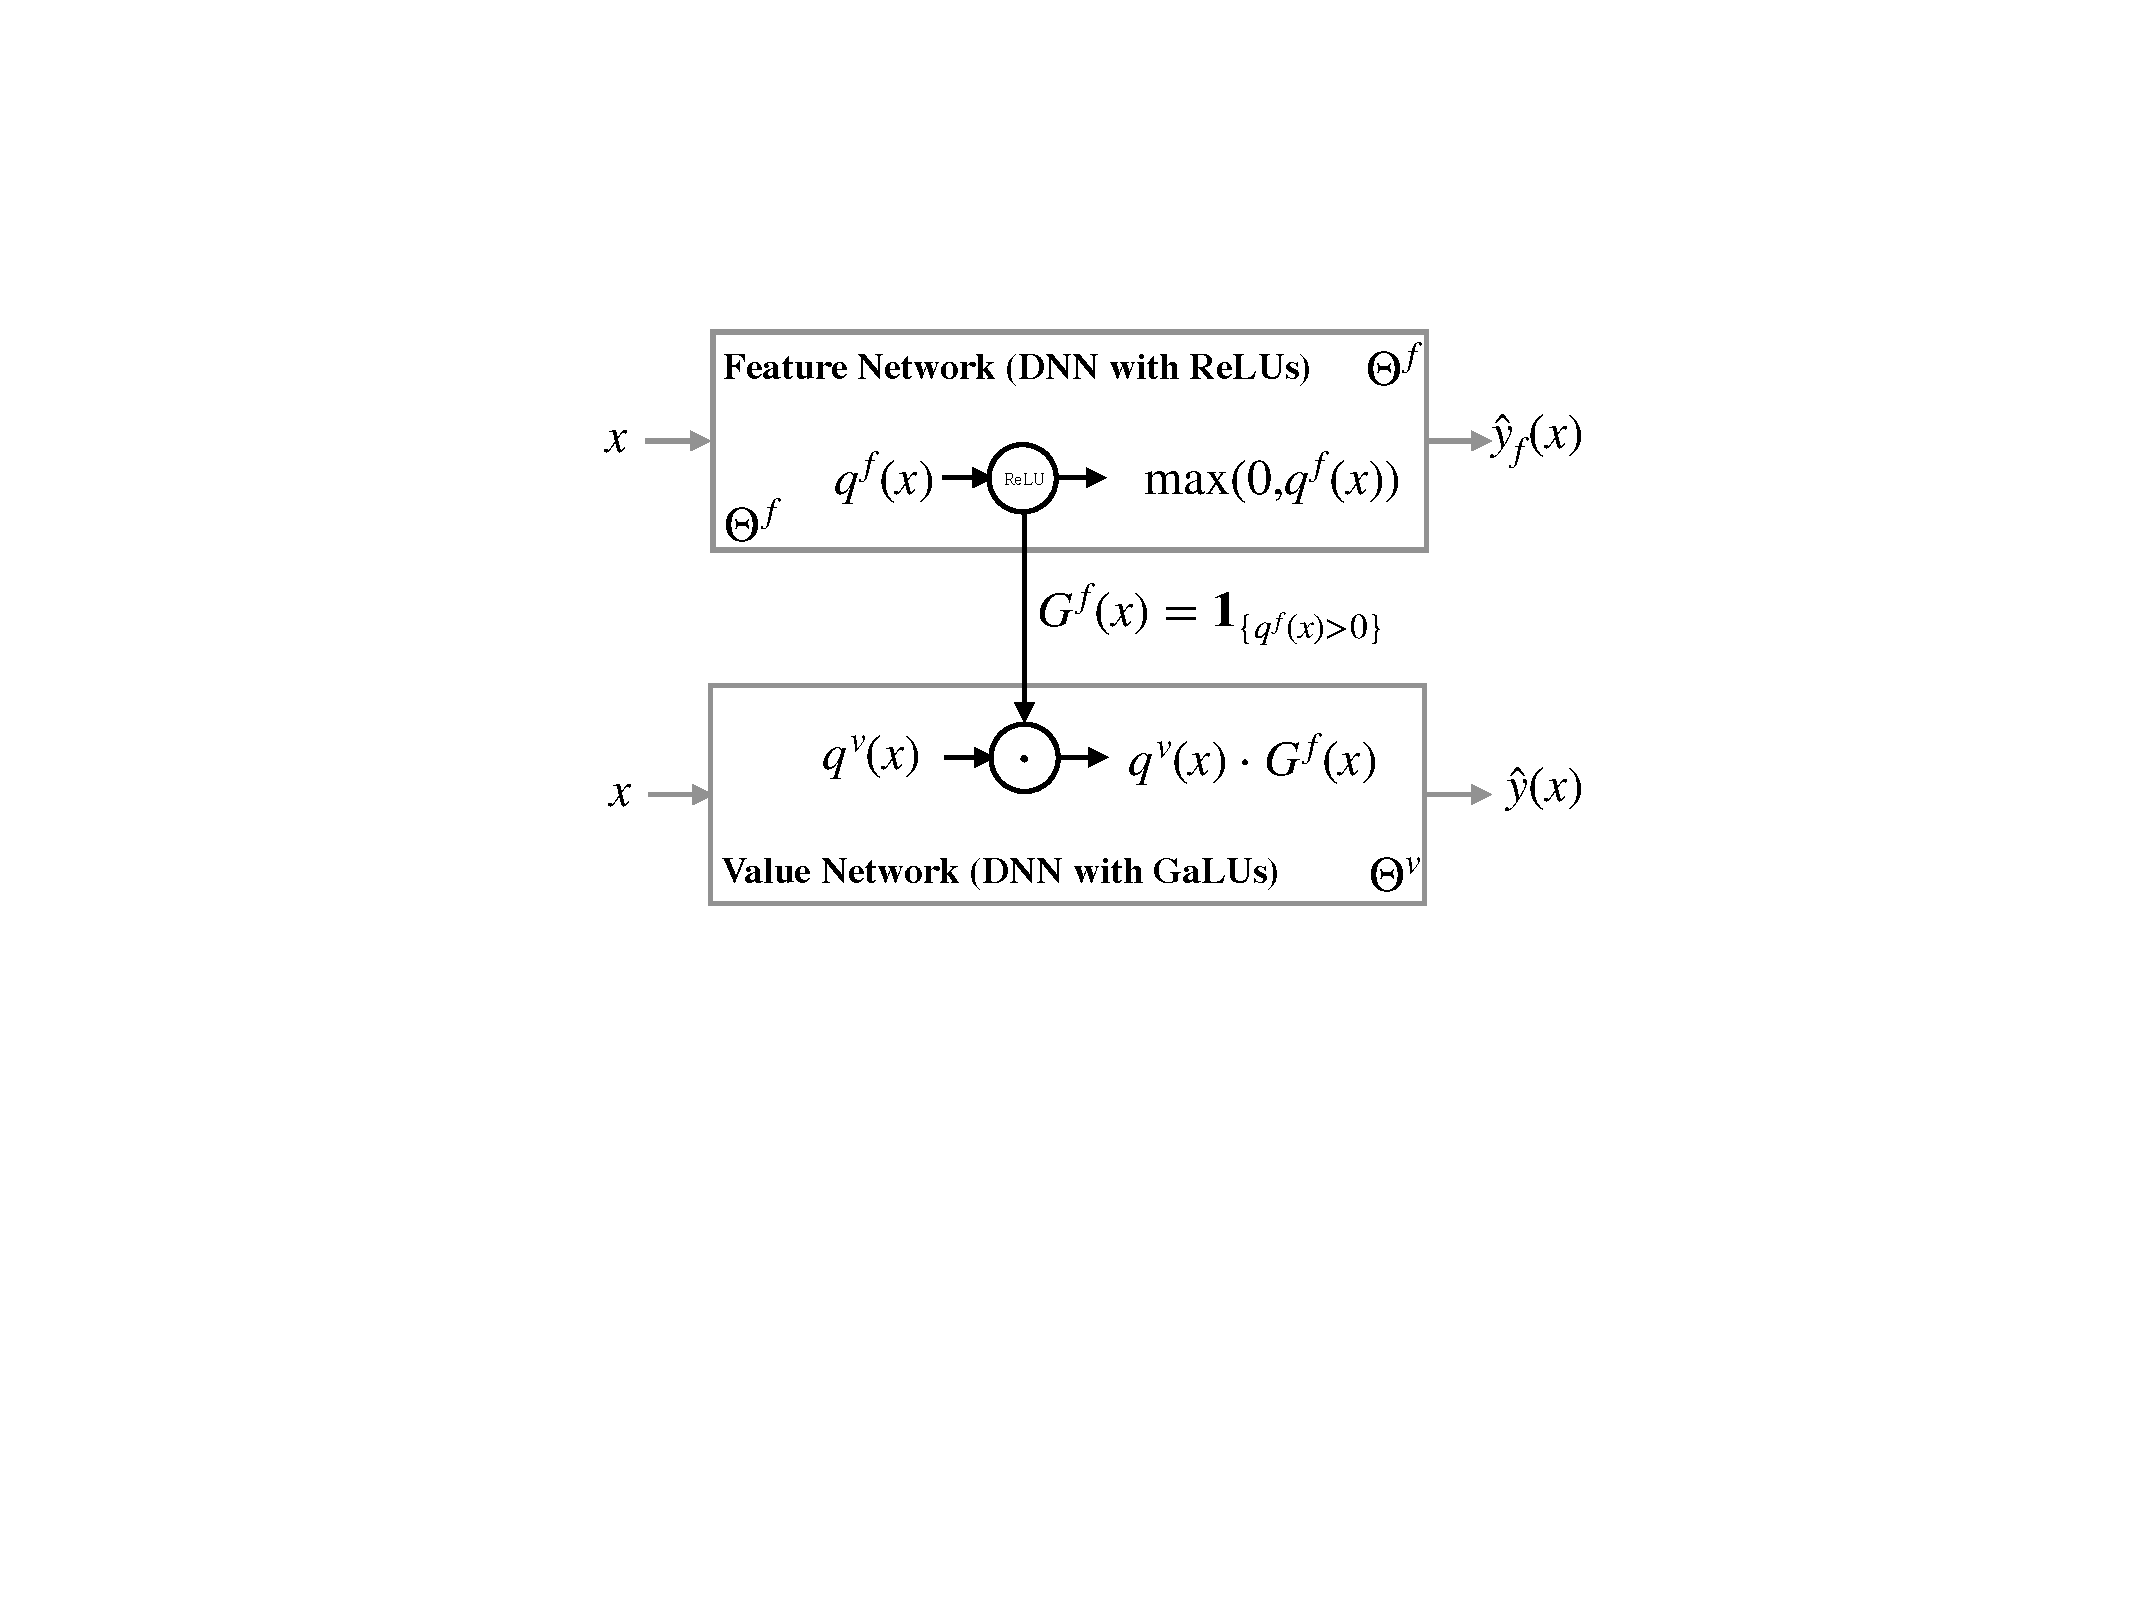
\includegraphics[scale=0.25]{figs/dgn-nips.pdf}
\end{minipage}
\begin{minipage}{0.6\columnwidth}
%\resizebox{\columnwidth}{!}{
\begin{tabular}{|c|c|}\hline
Regime & Feature Network \\\hline
Fixed Learnt & pre-trained; non-trainable \\\hline
Fixed Random & random; non-trainable\\\hline
Decoupled Learning & trainable \\\hline
\end{tabular}
%}
%\begin{tabular}{|c|c|}\hline
%Gating & Expression \\\hline
%Hard & $G^\text{f}(x) = \mathbf{1}_{\{q^{\text{f}}(x)>0\}}$ \\\hline
%Soft &  $G^\text{f}(x) = 1/(1+\exp{-\beta q^{\text{f}}(x)})$\\\hline
%\end{tabular}
%\resizebox{\columnwidth}{!}{
%\begin{tabular}{|c|c|}\hline
%NTK & $K_{\Tdgn}(x,x')=\ip{\nabla_{\Tdgn}\hat{y}(x),\nabla_{\Tdgn}\hat{y}(x')}$\\\hline
%Kernel & Expression\\\hline
%$\text{NTK}^{\text{gate-learn}}:$ & $\kf_{\Tdgn}(x,x')=\ip{ \nabla_{\Tf}\hat{y}(x), \nabla_{\Tf}\hat{y}(x') }$\\\hline
%$\text{NTK}^{\text{fixed-gate}}:$ & $\kv_{\Tdgn}(x,x')=\ip{ \nabla_{\Tv}\hat{y}(x), \nabla_{\Tv}\hat{y}(x') }$,\\\hline
%\end{tabular}
%}
\end{minipage}
\caption{Deep Gated Network }
\label{fig:dgn}
\end{figure}
\end{comment}
\begin{proposition}\label{prop:ntks} Let $\kv_{\Tdgn}(x,x')=\ip{ \nabla_{\Tv}\hat{y}(x), \nabla_{\Tv}\hat{y}(x')}$, and  $\kf_{\Tdgn}(x,x')=\ip{ \nabla_{\Tf}\hat{y}(x), \nabla_{\Tf}\hat{y}(x') }$ and $K_{\Tdgn}$ be the NTK matrix of the DGN. Then 
\begin{align*}
K_{\Tdgn}=\kv_{\Tdgn}+\kf_{\Tdgn}
\end{align*}

\end{proposition}
\textbf{Remark:} In the case of fixed regimes, $\kf_{\Tdgn}=0$. 

